\documentclass[12pt]{texmemo} % originally by Rob Oakes; adapted by Alice Chen and now Jacob Child

\memoto{ Adam Cardoza, Graduate Student in the BYU FLOW Lab}
\memofrom{Jacob Child}
\memore{Findings from the DJI II Trade Study}
\memodate{\today} % or \today
\memosection{497R (Andrew Ning)}

\begin{document}
\maketitle

\highlight(Intro of what I will be describing in the paper) ?
*there are too many plots, include a few and put the rest attached below?
A set of custom code heavily utilizing the CCBlade.jl package was A DJI II propeller was imported, analyzed, and it

*When and why do I limit things and how do the parameters influence the design space!

RVar findings

CVar findings

PVar findings

In each of the above discuss the effects on thrust, power, and figure of merit

Extra discussion on the Surface plots

Attachments
*do I put extra plots and code etc here?





Section II identifies three major problems with software patents in the U.S.:
\setlength{\parskip}{0pt} % no new line in list
\begin{itemize}
    \item The slow process in getting a software patent application reviewed and decided upon;
    \item The low quality of granted software patents in general; and
    \item The difficulty of challenging bad software patents efficiently.
\end{itemize}
\setlength{\parskip}{0.5\baselineskip plus 2pt} % reset

Section III dives into three policy suggestions of varying degrees of radicalness for implementation at the USPTO:
\setlength{\parskip}{0pt} % no new line in list
\begin{itemize}
    \item Roll out clearer guidelines for granting or rejecting software patents;
    \item Strengthen collaboration with the tech community, universities, and law schools; and
    \item Invest in an internal information technology (IT) system revamp in view of the growing power of artificial intelligence (AI).
\end{itemize}
\setlength{\parskip}{0.5\baselineskip plus 2pt} % reset

Finally, Section IV concludes this memo with the limitations of the policies suggested and their implications beyond software patents.

\section{RVar findings}

The purpose of this section is 

\textit{Statutory Patentability.} Patent examiners at the USPTO grant or reject patent applica

\textit{Subject Matter Eligibility.} It is unclear from the Patent Act whether and which software pat


\textit{Opposition Procedures.} The USPTO currently offers several ways of 
\section{PVar Findings}

In this section I flesh out three major issues with software patents.

\textit{Slow Process.} It takes near

\textit{Low Quality.} Granted software

\textit{Costly Opposition.} If it is hard to ensure that granted patents are generally of high q

\section{CVar Findings}

In this section I propose three policies t

\textit{Clearer Guidelines.} tware patents and the tug-of-war between the SCOTUS and the CAFC, patent examiners and administrative law judges at the US

\textit{Stronger Collaboration.} \cite{lee} More and more students are majoring in computer science, more and more people are getting involved in open-sou 

\textit{Smarter System.} Modernizing the IT system 

\section{Surface Discussion}
filler bla bla baa

\section{Conclusion: Overall trends and implications, further research}

What the USPTO can do is limited. 

\newpage
\printbibliography

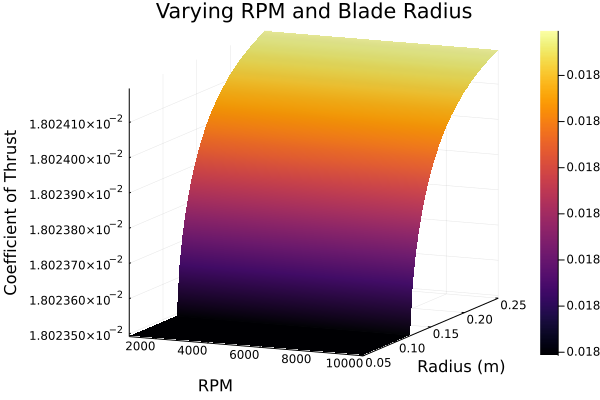
\includegraphics[scale=.65]{./surfaces/RVarCTSurfacePlot}
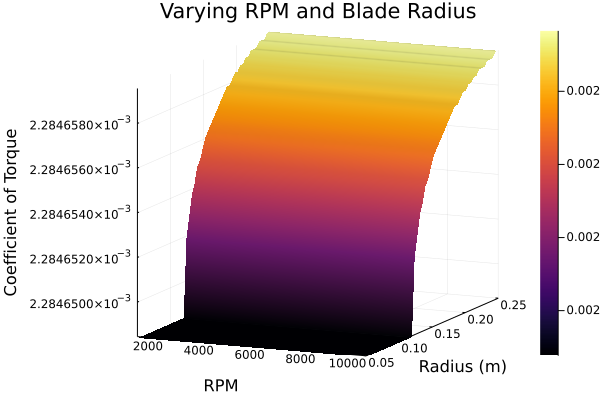
\includegraphics[scale=.65]{./surfaces/RVarCQSurfacePlot}
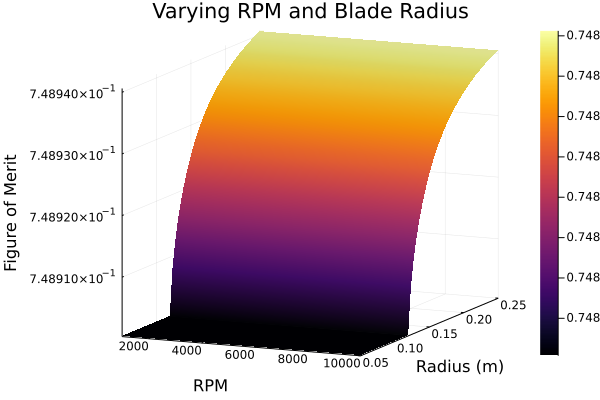
\includegraphics[scale=.65]{./surfaces/RVarFMSurfacePlot}
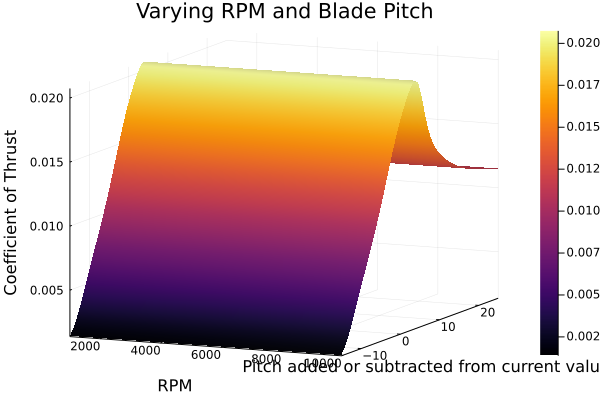
\includegraphics[scale=.65]{./surfaces/PVarCTSurfacePlot}
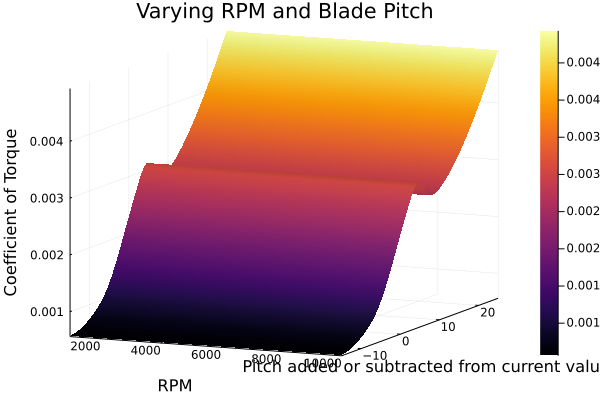
\includegraphics[scale=.65]{./surfaces/PVarCQSurfacePlot}
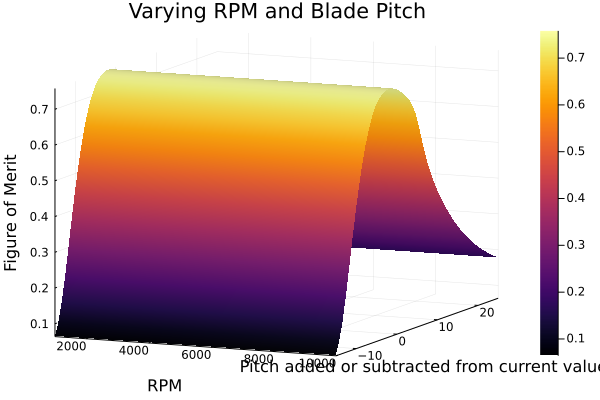
\includegraphics[scale=.65]{./surfaces/PVarFMSurfacePlot}
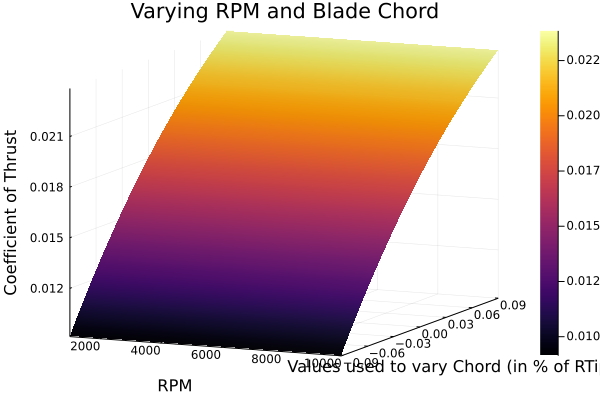
\includegraphics[scale=.65]{./surfaces/CVarCTSurfacePlot}
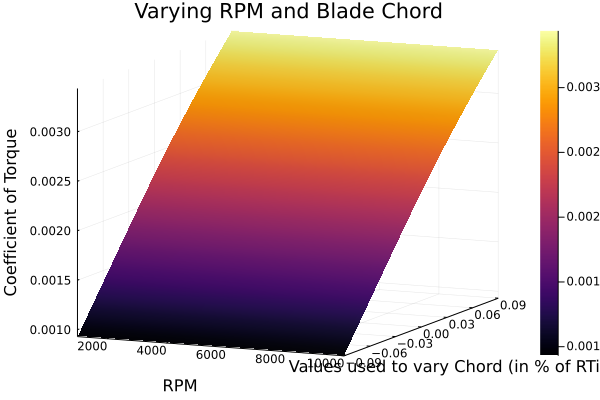
\includegraphics[scale=.65]{./surfaces/CVarCQSurfacePlot}
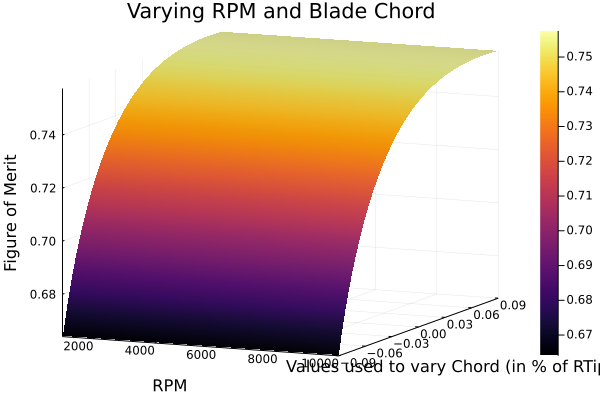
\includegraphics[scale=.65]{./surfaces/CVarFMSurfacePlot}
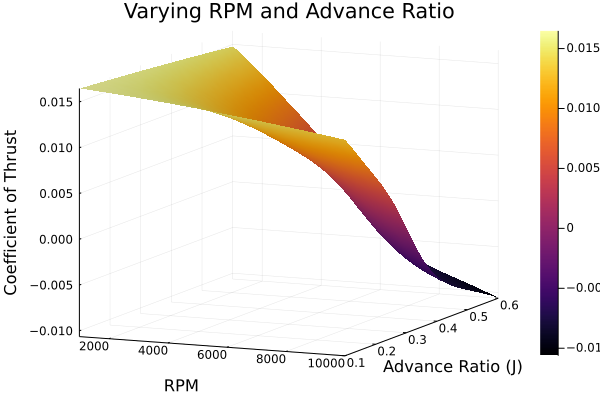
\includegraphics[scale=.65]{./surfaces/JVarCTSurfacePlot}
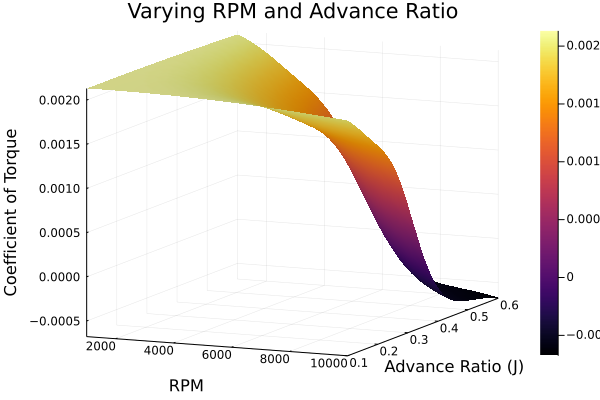
\includegraphics[scale=.65]{./surfaces/JVarCQSurfacePlot}
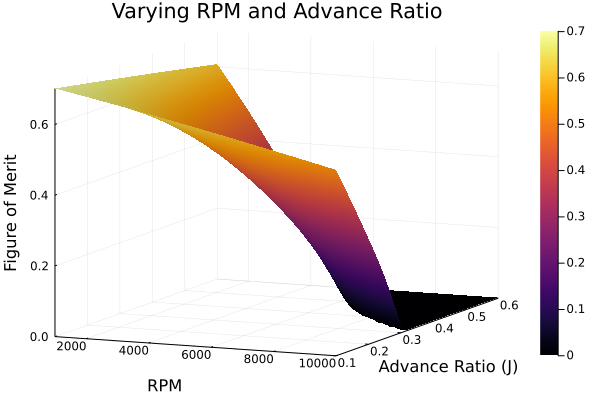
\includegraphics[scale=.65]{./surfaces/JVarFMSurfacePlot}
\end{document}